\documentclass{article}

\usepackage{microtype}
\usepackage{hyperref}
\usepackage{pdfpages}
\usepackage{float}
\usepackage{graphicx}

\title{COMP1002 Assignment\\Documentation}
\author{Jakob Wyatt\\19477143}

\begin{document}
\maketitle
\pagebreak
\section{Overview}
\label{sec:Overview}
This program is designed to simulate a social network.
The entry point of the program can be found in \texttt{src/SocialNetworkSim.py}.
The user interface is as specified in the assignment brief,
with additional functionality including graphical representation
of the socical network in interactive mode (\texttt{display}), and interactive liking/unliking 
of posts. An example of this graphical representation is shown below.\\
\begin{figure}[H]
\centering
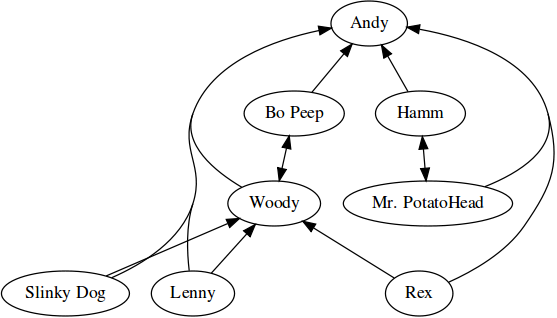
\includegraphics[width=.7\linewidth]{display}
\end{figure}
There exists only one post at a time, with a new post being loaded when the current
post has not had any activity in the last timestep. The original poster always
likes their own post. A user can only like a post once.\\
The simulation consists
of timesteps, with a function \texttt{update()} to move between timesteps.\\
The social network consists of a set of users that may follow eachother,
which has been represented in code as a directed graph. Users may not follow themselves,
or follow eachother more than once.\\
The update algorithm works as follows:
\begin{enumerate}
    \item Check that there exists some users that have liked the post in the previous timestep.
            If there are none, the update ends and the next post is loaded.
    \item Iterate through all users who liked the post in the previous timestep.
            Each of their followers is 'exposed' to the post, and have a chance of liking the post.
            This chance is sampled from a Bernoulli distribution with probability
            $\mathit{clamp}(\mathit{prob\_like} \times \mathit{clickbait\_factor}, 0, 1)$.
    \item If a user likes a post in the current timestep, they have a chance of following the
            original poster. This is sampled using the same technique as above, with global probability
            $\mathit{prob\_foll}$.
\end{enumerate}
Note that in the above algorithm, if a user does not like a post, they may potentially
be exposed to it later via a different friend. This behaviour is intentional, as it incentivises
a highly connected network.

It should be noted that all class fields and data structures use DSA
ADTs/Data Structures for implementation. However, within individual methods,
some python data types such as List have been used, to help enhance code clarity
when performing some operations. This minor use of python data structures
has been approved by Ben, my DSA Tutor.

For command line argument parsing and an interpreter-style user interface
in interactive mode, the python modules \texttt{argparse} and \texttt{cmd}
were used. This has also been approved by Ben.

\section{UML}
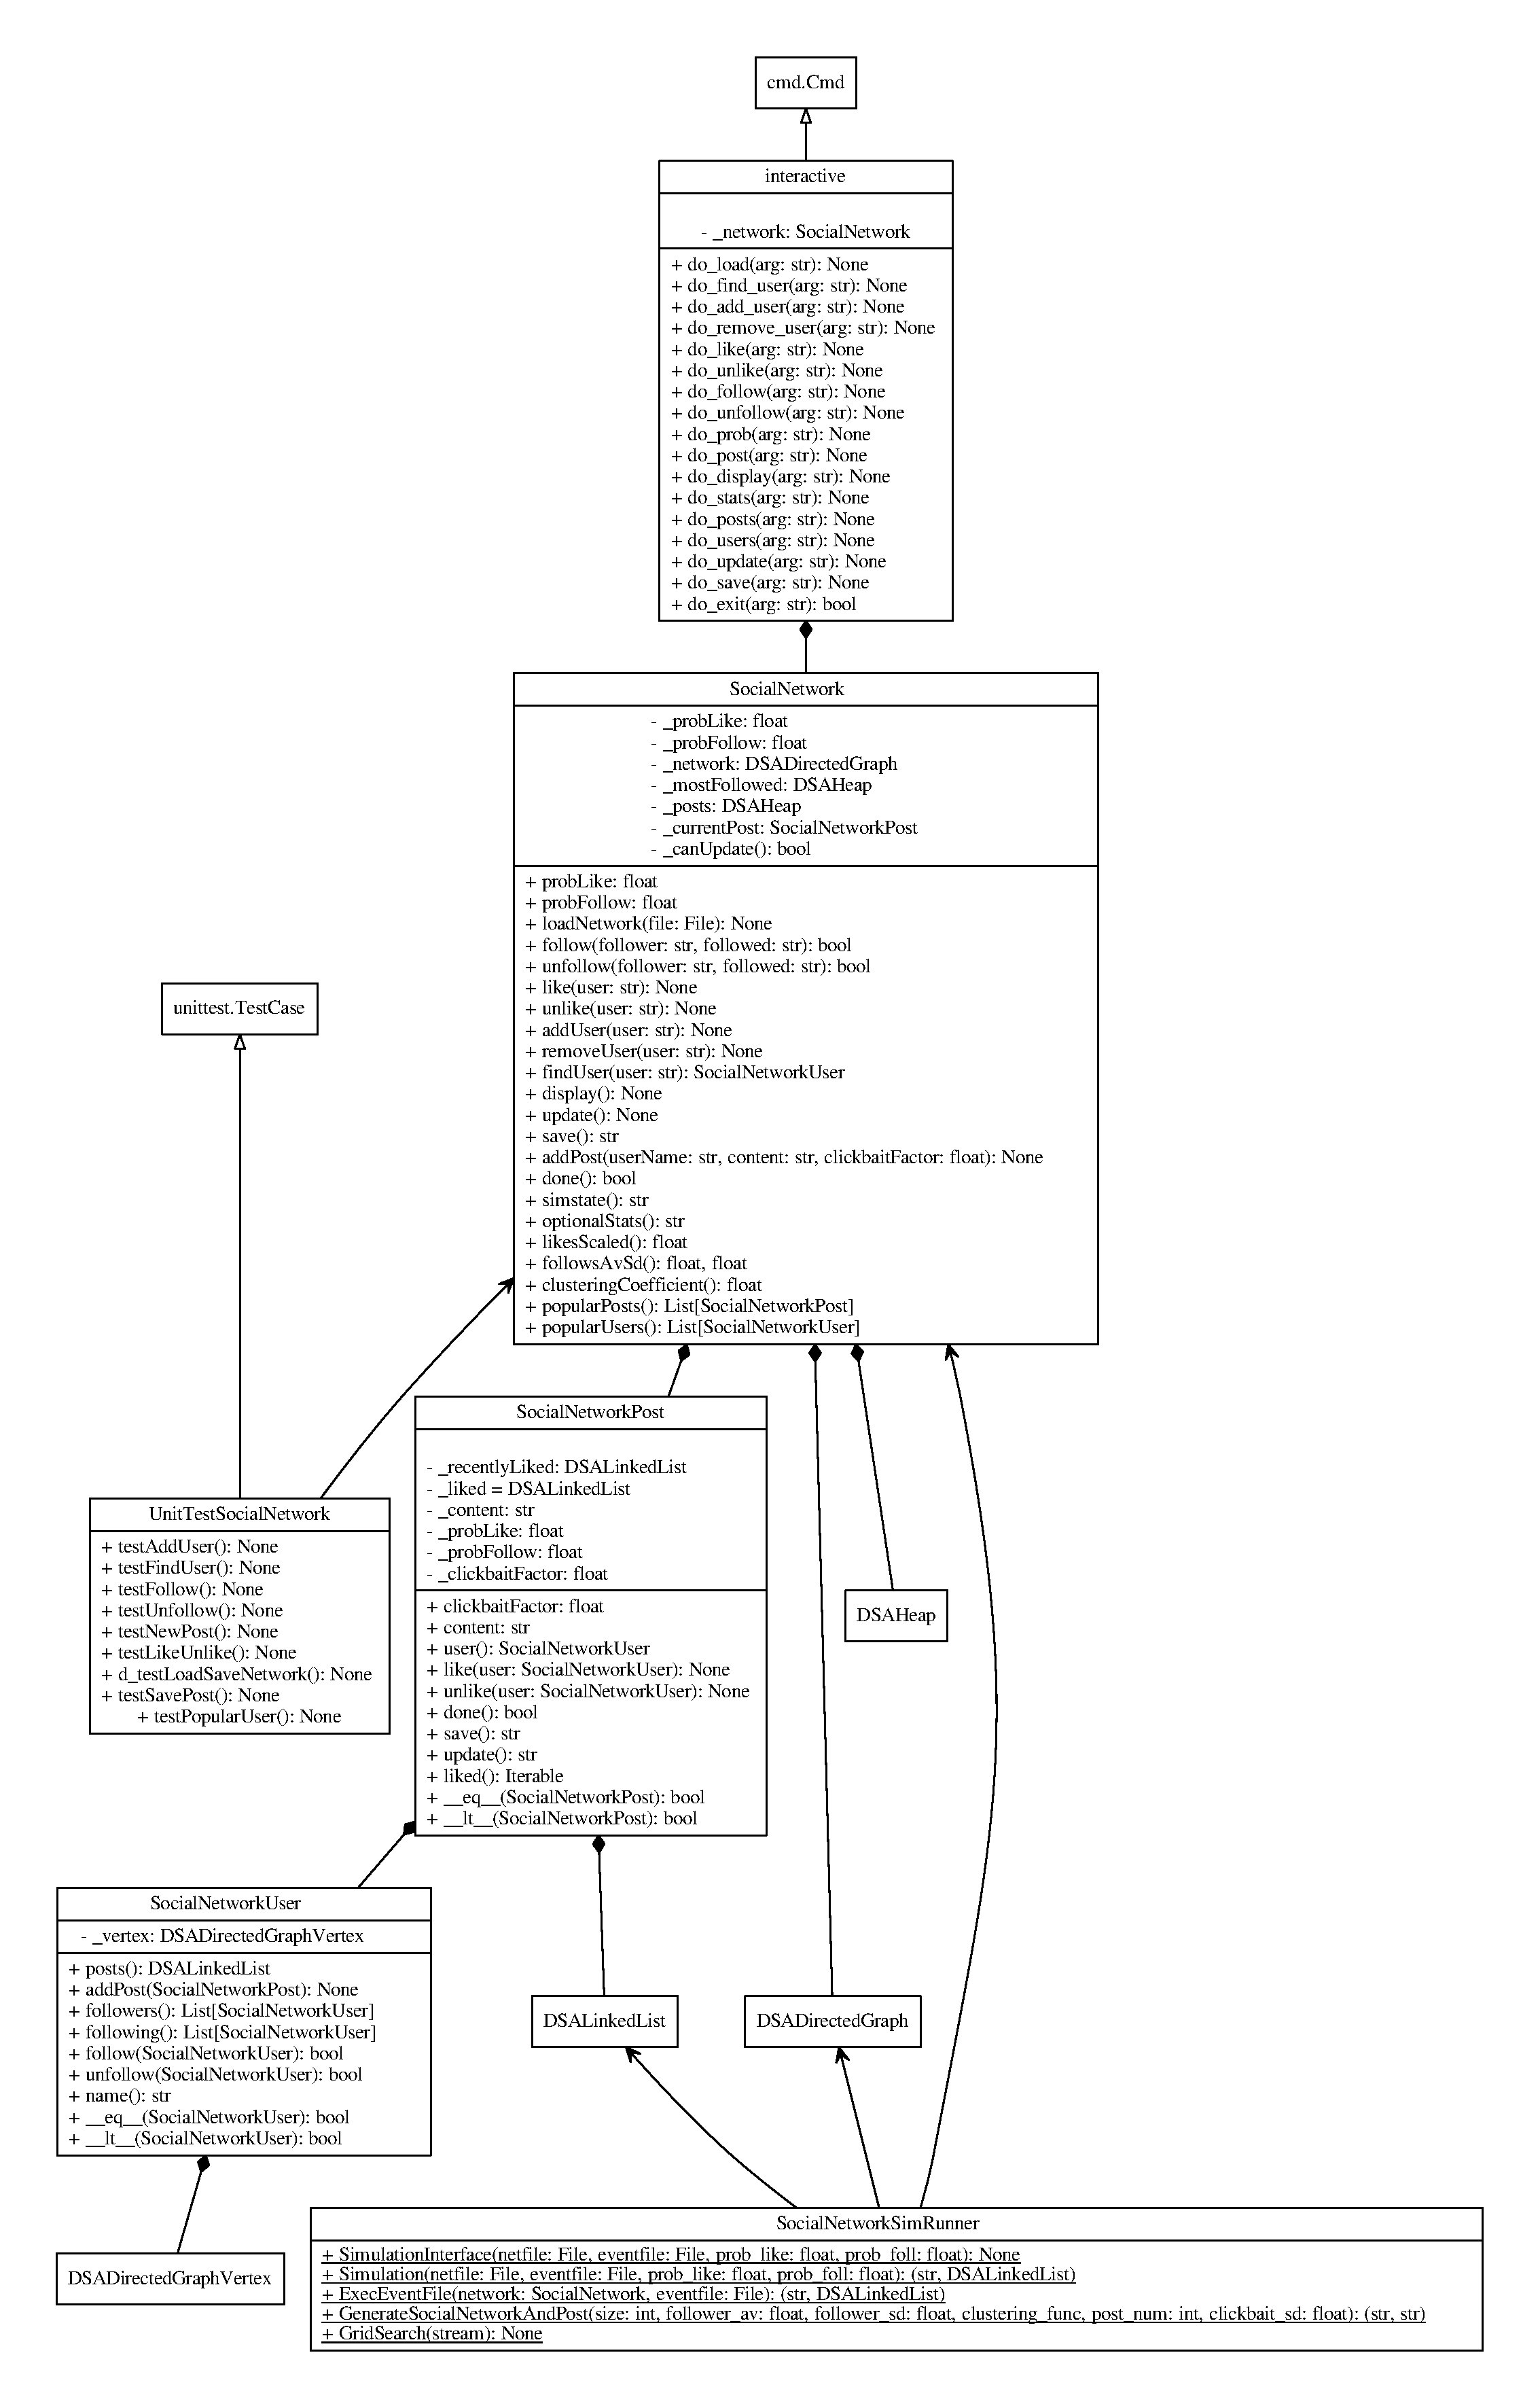
\includepdf{UML.pdf}
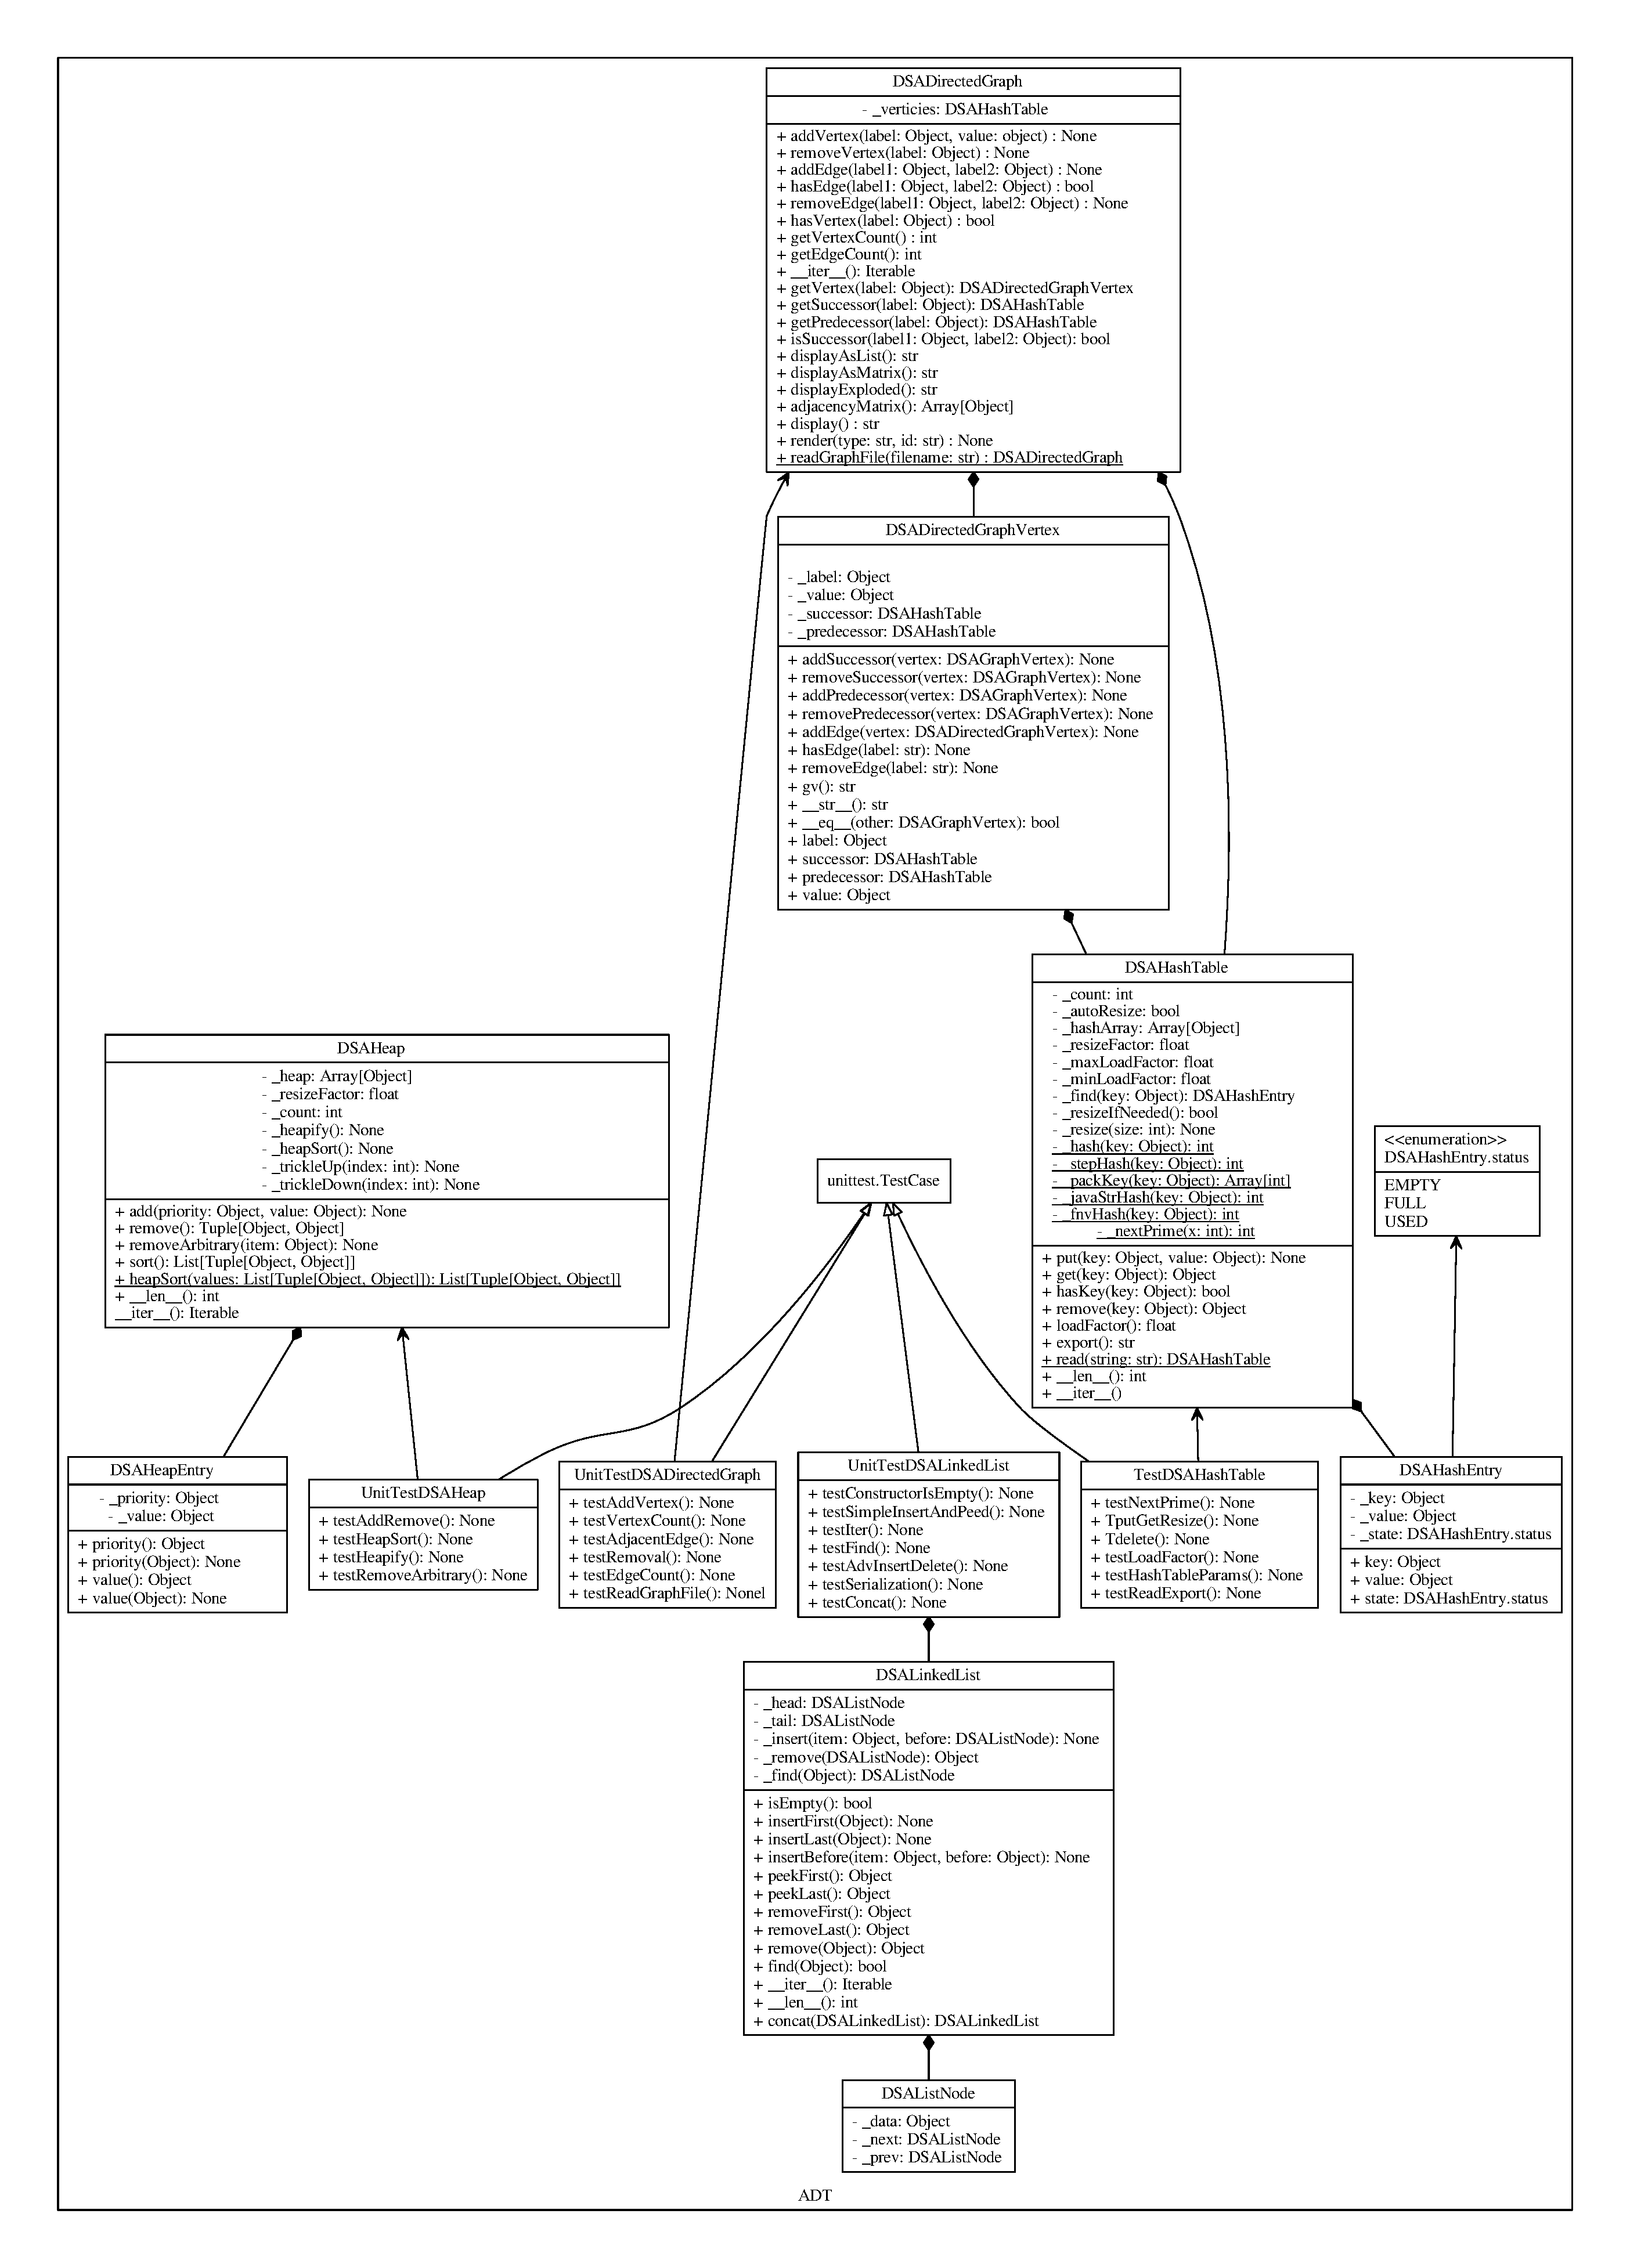
\includepdf{UML_ADT.pdf}

\section{Classes}

Unit test classes have been excluded from this section,
as they are all similar. Each unit test class inherits from python's \texttt{unittest.TestCase} class,
and have been created to test class X, where the name of the test class is
\texttt{UnitTestX}.

\subsection{SocialNetworkCore.SocialNetwork}
This class contains an interface for creating and updating a social network,
and contains common functionality used in both interactive and simulation mode.
By doing this, the underlying data structures used to store the network
can be changed without needing to also change the user interface code.
Data structures used in this class are explained in \autoref{sec:Justification}.

\subsection{SocialNetworkInteractive.interactive}
This class inherits from the python \texttt{cmd.Cmd} class
to implement an interactive interpreter-like interface for the program.
It uses the \texttt{SocialNetworkCore.SocialNetwork} class for storage and manipulation of the social network.

\subsection{SocialNetworkPost.SocialNetworkPost}
This class represents a post on the social network,
and can be queried to obtain the users that have liked the post, the original poster,
and the post content. It also contains a method \texttt{update()},
which propogates the post through the network by one timestep.
The core of the propogation algorithm is implemented in this method.

\subsection{SocialNetworkUser.SocialNetworkUser}
This class is a wrapper around a DSADirectedGraphVertex that has been created
by the SocialNetwork class. As such, it does not store any data internally,
and performs most functionality by calling corresponding functions within the DSADirectedGraphVertex class.

The reason why this class was created was to create a wrapper around the
DSADirectedGraphVertex class, using terms specific to social networks.
This allows the DSADirectedGraph class to remain generic for future use.

Another advantage is that this class can be returned from functions within
the SocialNetwork class, which creates an external interface for user specific
functionality. This means that the underlying implementation of a user may be
changed without breaking any code that uses the SocialNetworkUser class.

\subsection{ADT.DSADirectedGraph.DSADirectedGraph}
This class is an ADT of a directed graph, and contains functionality to add/remove verticies and edges from the graph.
The class uses terms from graph theory such as "successor" and "predecessor"
so that it can remain use agnostic, and can be carried over to other projects
that may require a graph implementation.
It is currently implemented using the \texttt{DSAHashTable} data structure,
however it has been implemented using a \texttt{DSALinkedList} in the past.
Reasons for this data structure choice have been explained in the \autoref{sec:Justification} section.

\subsection{ADT.DSADirectedGraph.DSADirectedGraphVertex}
This class contains information about a vertex, including its label, data, and edges.
This is a container class intended for use within the DSADirectedGraph class.

\subsection{ADT.DSAHashTable.DSAHashTable}
This class is an impementation of an automatically resizing hash table,
with $O(1)$ amortized insert, delete, and find operations.

\subsection{ADT.DSAHashTable.DSAHashEntry}
This class represents an entry in a \texttt{DSAHashTable},
and contains setters and getters for entry keys, values, and state.

\subsection{ADT.DSAHeap}
This class implements a max-heap using an array.
This gives $O\left(n\log n\right)$ sort and $O\left(\log n\right)$ insert/remove.
Resizing occurs automatically when the heap is too large.

\subsection{ADT.DSAHeapEntry}
This class is a convenience class for use within the \texttt{DSAHeap} class,
and represents a single entry in the heap.

\subsection{ADT.DSALinkedList}
This class implements a doubly linked, doubly ended, linked list
with cached length. This linked list also supports list concatenation
in $O(1)$ time.

\subsection{ADT.DSAListNode}
This class is used to represent an entry inside the DSALinkedList class.

\section{Justification}
\label{sec:Justification}
In any program, whenever an ADT or algorithm is selected for use, this use must be justified.
Choice of an ADT must help enhance clarity, make implementation of an algorithm easier,
and have good time and space complexity.\\

\subsection{Data Structure Selection}

The user network uses the \texttt{DSADirectedGraph} class to represent follows between users
as edges. This helps to enhance clarity, as follows between users are inherently directional in nature.\\

Operations that must be performed within this directed graph are find/add/remove verticies,
and find/add/remove edges. It should also be noted that within the context of a social network,
there exists a maximum of one directed edge between any 2 nodes. Duplicate nodes also will not
exist.
To store verticies and edges within this directed graph, the \texttt{DSALinkedList} class was originally
used to store this data. However, this ended up being rather inefficient, with a time complexity of
$O\left(V\right)$ for vertex find/remove and $O\left(E + V\right)$ for edge find/remove.
Although vertex add and edge add are theoretically $O\left(1\right)$, in practice they had a time complexity
equal to vertex find and edge find, as it had to be checked that the vertex/edge did not already exist in the network.\\

To improve the performance of these operations, a DSAHashTable was used to store the verticies and edges instead.
This gives $O\left(1\right)$
performance for find, insert, and remove operations. Despite the greater overhead, in practice it was found to outperform
the linked list implementation at a graph size of 20, and approximately doubled the speed when the number of verticies was 50.\\

Multiple \texttt{SocialNetworkPost} objects need to be stored within the \texttt{SocialNetwork} class.
The only time all posts need to be accessed
is when the class is queried for popular posts, which requires ordering the posts by likes.
A simple sorting approach will have a time complexity of $O\left(n\log n\right)$. However, this
approach requires resorting all posts every time the function is called.\\

Storing the posts in a \texttt{DSAHeap} still maintains
the time complexity of $O\left(n\log n\right)$ when sorting. However, if \texttt{popularPosts}
is called multiple times, the DSAHeap is already in a sorted state, which greatly reduces the execution time.
A class field is used to cache the most recent post.\\

As well as being stored in the \texttt{DSADirectedGraph}, users are also stored in a \texttt{DSAHeap},
sorted by follower count. This is done to increase the efficiency of the popular users operation,
as the users are always stored in a semi-sorted state.
One disadvantage of this strategy is that it increases the memory footprint. However, it only increases it
by a linear factor, and does not change the space complexity of the program.\\

Another performance optimization is that user posts are cached in a dedicated linked list per user.
When finding all of a users posts, this gives a significant performance increase,
as only a small subset of the total posts need to be iterated over.\\

\subsection{Alternative Timestep Algorithms}

An alternative post propoagtion algorithm to the one described in \autoref{sec:Overview}
is to use a breadth first search through the graph instead,
iterating over all the nodes in the network exactly once. The reason why this was decided against was because
the desired behaviour was to expose a user to a post more often if more of their friends interacted with the post.
This emulates behaviour on social media
platforms such as facebook, where a user may see an old post if a friend has recently liked it.\\

\subsection{Clustering Coefficient}

Some other interesting algorithms that were implemented in this program is the calculation of the globally averaged local clustering coefficient, found in the
function \texttt{SocialNetwork.ClusteringCoefficient}.
This allows analysis of of how well connected a group of users is.
To calculate the clustering coefficient of a vertex $V$, the neighbourhood of that
vertex is first found.\\
$N = V_{successors} \bigcup V_{predecessors}$\\
Next, the number of connections between nodes in this neighbourhood is found.\\
$C = |{e_{jk} : v_j, v_j \in N, e_{jk} \in E}|$\\
Finally, this is divided by the total number of potential connections within the neighbourhood.\\
$\mathit{Clustering Coefficient} = \frac{C}{|N| \times (|N| - 1)}$\\
To find the network average clustering coefficient, the clustering coefficient
is calculated for all verticies in the network and averaged.
As the number of followers will always increase over time in this simulation,
to enable comparison between clustering coefficients at different timesteps,
the network average clustering coefficient was then divided by the number
of edges in the graph.
This algorithm has $O\left(n^3\right)$ execution time when hashtables are used to store
edges and verticies, as is done in this program. When a linked list is used instead, this execution time jumps to
$O\left(n^4\right)$.\\

\subsection{Network Generation}

To generate the simulated networks, a unique algorithm was used
that was created by the author, and to their knowledge, does not exist anywhere else.
This algorithm allows efficient generation of structured (non-random) networks,
with a consistent runtime complexity of $O\left(V \times E\right)$.

First, a number of verticies are created.
Next, these verticies are iterated over, and the number of successors of each
vertex is calculated by sampling from a distribution $X \sim N\left(follower\_av, follwer\_sd^2\right)$.

To select the edges of the network, an approach was used that is similar in concept
to a variogram, used in the field of geostatistics.
A variogram measures the amount of correlation between two points in a field that are some distance apart.
In this algorithm, this distance is discrete rather than continuous, and is measured by finding
a path between two nodes. By increasing the correlation between nodes at short distances,
a graph can be created with a higher clustering coefficient. Alternatively,
decreasing the correlation between nodes causes the graph to become more randomised,
and less clustered.

The clustering coefficient of a vertex can be generalized to include all verticies
within some distance $h$ of a central vertex (Xiao et al. 2007), rather than
only verticies within a distance of 1 of the central vertex.

In a social network, it is reasonable to assume that the clustering
coefficient will decrease as the distance increases.
One way to visualise this is that your friends are likely to be interconnected,
whereas your friends of friends are less likely to be interconnected directly.
By creating graphs that follow this property, realistic social networks
can be created for use in simulations.

To generate an edge in the graph, a random walk is performed starting at a given vertex, $V_0$.
This random walk occurs along any nodes that are predecessors of the current node,
and does not loop back onto previously visited nodes.
At each step on the random walk, the probability of creating an edge between the current node and $V_0$
is calculated by evaluating the variogram $\gamma (h)$, where h is the distance that has been travelled on the random walk.

If an edge is created, a new random walk begins starting at the vertex $V_0$,
and this algorithm repeats until the correct number of edges have been created
for this vertex.
If there are no valid verticies to walk to,
or the random walk has reached some distance threshold from the original node,
an edge is created with any random vertex in the graph. This allows initial
'bootstrapping' of the network when no edges have yet been created.\\

\subsection{Gridsearch}

To profile multiple runs of the simulation a gridsearch algorithm was used
to vary the below parameters:
\begin{itemize}
\item Average and s.d. of followers per user
\item Like/Follow probabilities
\item Number of users in the network
\end{itemize}

First, arrays that contain the parameter values to be tested were created.
Next, for all possible combinations of these parameters, a network
matching these parameters was created. A simulation was then run on all networks,
with simulation statistics being logged to a file in CSV format.

Parameters that are varied during the gridsearch include the like and follow probabilities,
network size, clickbait standard deviation, and
follower average / follower standard deviation.

An advantage of this algorithm is that it is very simple to implement.
However, a disadvantage is that it takes a long time to execute when there are many input parameters.
The algorithmic complexity of the gridsearch algorithm
is $O(x^n)$, where n is the number of parameters that are varied and x is the number
of datapoints per parameter.

\end{document}
